% Created 2017-10-03 Tue 20:01
% Intended LaTeX compiler: pdflatex
\documentclass[12pt]{scrartcl}
\usepackage[utf8]{inputenc}
\usepackage[T1]{fontenc}
\usepackage{graphicx}
\usepackage{grffile}
\usepackage{longtable}
\usepackage{wrapfig}
\usepackage{rotating}
\usepackage[normalem]{ulem}
\usepackage{amsmath}
\usepackage{textcomp}
\usepackage{amssymb}
\usepackage{capt-of}
\usepackage{hyperref}
\author{Xiong ChenYu \\
U1521516C \\
EEE \\
}
\date{May 16, 2017 \\
}
\title{
\includegraphics[width=\textwidth]{img/NTU.png} \\
[3\baselineskip] REPORT \\
ON \\
INDUSTRIAL ATTACHMENT \\
WITH \\
ELEOS WEB PTE.LTD \\
[3\baselineskip]}
\hypersetup{
 pdfauthor={Xiong ChenYu \\
U1521516C \\
EEE \\
},
 pdftitle={
\includegraphics[width=\textwidth]{img/NTU.png} \\
[3\baselineskip] REPORT \\
ON \\
INDUSTRIAL ATTACHMENT \\
WITH \\
ELEOS WEB PTE.LTD \\
[3\baselineskip]},
 pdfkeywords={Intership Report},
 pdfsubject={},
 pdfcreator={Emacs 27.0.50 (Org mode 9.1.1)},
 pdflang={English}}
\begin{document}

\maketitle
\tableofcontents

\listoftables
\listoffigures

\newpage
\section{Abstract}
\label{sec:org52b434c}
This report describes the internship I spent at the ELEOS WEB PTE.LED. The
ELEOS WEB PTL.LES is a web company provide solution for retailer management.
They provide lots of products.
\begin{itemize}
\item Octopus\(^{\text{TM}}\) Retail POS :

\begin{quote}
A Comprehensive Retail Management Solution
Complete, easy-to-use, stand-alone POS solution specially designed for small
and medium scale retail businesses such as clothing stores, electronic
computer stores, pharmacies drug stores and almost any other retail stores.
Integrates perfectly with your desktop, laptops or mobile devices.
\end{quote}

\item Octopus\(^{\text{TM}}\) Food POS :
\begin{quote}
\textbf{A "Smart" Cafe-Experience}  \\
Octopus™ Food POS is an ideal choice for F\&B outlets. Connecting the
Point-of-Sales device with the rest of your other devices – OctoWaiter, OctoMenu
and self-service kiosk seamlessly, Octopus™ Food POS provides a modern seamless
concept and high efficiency for your F\&B operations.
\end{quote}

\item E-Commerce :
\begin{quote}
Break Geographical Barriers. Reach Out to Your Potential Customers. \\
\textbf{Octopus\(^{\text{TM}}\) E-Commerce} replicates your offline business into online business
literally in minutes. Armed with a powerful management interface, Octopus™
E-Commerce allows users to manage their own virtual stores easily, including
management of images, setting up promotion activities and monitoring of your
inventory and customers from an integrated standpoint.

\begin{itemize}
\item YOUR BUSINESS NEVER SLEEPS :
\end{itemize}
Get your business to work for you even when you are asleep or on vacation.
Publish your products / services and start an online presence.

\begin{itemize}
\item GO BORDERLESS :
\end{itemize}
Break out from your market and bring your business to the international level.
See how our solutions can enhance your market reach and customer base.

\begin{itemize}
\item POS-CONNECTED HASSLE-FREE PRODUCT INPUT :
\end{itemize}
Add in product easily from your existing POS product database. Or opt to input
new or online-exclusive products via web access. Makes inventory management easy.

\begin{itemize}
\item FUSS-FREE CONTENT MANAGEMENT :
\end{itemize}
Choose your preferred theme, customise the layout and you are ready to sell
online. Simple interface allows you to insert your company logo; create new
pages, page navigation and product blogs easily. No prior programming skills needed.
\end{quote}

\item Companion Apps :
\end{itemize}
\begin{quote}
\begin{itemize}
\item Octopus™ Mobile POS :
\end{itemize}
Point of Sales with Mobility in Mind

POS is now even more compact for your phone. Octopus™ Mobile POS is a complete
all-in-one solution that is ideal for retailers and consumer merchants alike.

\begin{itemize}
\item Octopus™ Admin Dashboard :
\end{itemize}
Pulse for Your Business
Octopus™ Admin Dashboard gives the business owners their key performance
indexes - whether it is their sales revenue, best sellers or what colour sells best in which season.

With Octopus™ Admin Dashboard, business owners have the pulse of their business at their finger tips.
\end{quote}

\newpage
\section{Acknowledgment}
\label{sec:org27a8bb0}
First I should thank Nanyang Technology University gives me a change to have
the internship experience. \\
Second I should thank my supervisor Mr. Drake, he gives me a lot of freedom to
explore and learn new frameworks. \\
Thirdly I should thank Prof. Jong Ching Chuen who gave me a lot of advise during
the Internship. \\
Lastly I should thank all my fellows working in Eloes Web interns and formal
stuff. They help me a lot during the internship.

\newpage
\section{Chapter One}
\label{sec:orgc87e144}
\subsection{Introduction}
\label{sec:orgd68c741}
During my internship period, I work as Full-stack developer. My duty is to
develop a royalty and promotion system. The system consist 2 parts, one is
the android and ios application running on customers mobile device. They can
use the application to favorite the shops and get royalty points. What's more
they can also receive the E-stamps and get the new promotion notifications.
Another part is a AdminDashboard for the shop holders. They can use this to
add the new customers to their loyalty system and group them to distribute
the e-stamps, e-vouchers and push the promotion notifications.
\subsection{Background}
\label{sec:orga368f14}

I decide to use the most baised framework metoer witch have the most fastest
develop speed,so the can test the prototype easily,and make changes,and we use
the mongodb cause it is not schema based that means we can change the database
structure easilily and have the less side effect,despire we have to create the
customize schema on application level on my own .

The learning curve is good,first I do the 3 todo app on the official web and I
found the react version is more suitable for  the project cause in the future we
need the mobile version on android and ios so the react native is a better
choice.So build the react to our skill stack will save the future.

I need to develop the ios app,so I can not skip the mac os.But not all my notebook is mac to I need a stable system to develop the backend and frontend of the system.I used to be a Arch Linux user but It is just a platform for play with the linux, the community is quite ambicious.They always take the most latest as the rolling distribution.Another popular choice is geetoo wich also very clean.But the geetoo is souce based rather than binary based compared to arch which means the you can control the compiling process on you own so you need a high proformeance computer.

So I use elementary OS witch is based on ubuntu but it more like mac OS.The installing is very easy.Follow the official and you will get it easily.
I decide to choose a editor for my life change.The choice is firstly vim and then change to the nvim for the better economy of the synchronized api which makes the editor much faster and never block the ui.

I list all the all thins I used to create the application from front-end to
backend.

\begin{table}[htbp]
\caption{\label{tab:org793ea79}
The Usages and tools}
\centering
\begin{tabular}{ll}
Usages & Tools\\
\hline
Editors & Neovim, Emacs\\
Debugger & Google-Chrome\\
Backend Framework & MeteorJs\\
Front-end Framework & ReactJs\\
Front-Ui Framework & Meterial-Ui\\
Front-State Framework & Redux\\
Distribution Framework & Webpack 2\\
Database & MongoDb\\
Documentation & GitBook\\
\end{tabular}
\end{table}

\newpage

\section{Chapter Two}
\label{sec:orge1da213}
\subsection{Team Work}
\label{sec:orgee16887}
We use Github as the version control system to do the team work. We do the
different parts together and merge it to a single files. We use the github
branch to manage the new feature testing and gh-pages page to use the gihub
page to make documentation.
\subsection{Mobile Application}
\label{sec:orgc5cabec}
It is the Android and Ios application running on customers \hyperref[fig:org606d639]{\emph{mobile device}}. They can
use the application to \hyperref[fig:orgedc7f17]{\emph{favorite the shops and get royalty points}}. What's more
they can also receive the E-stamps and get the new promotion notifications.

\begin{figure}[htbp]
\caption{\label{fig:org606d639}
Login Page}
\centering
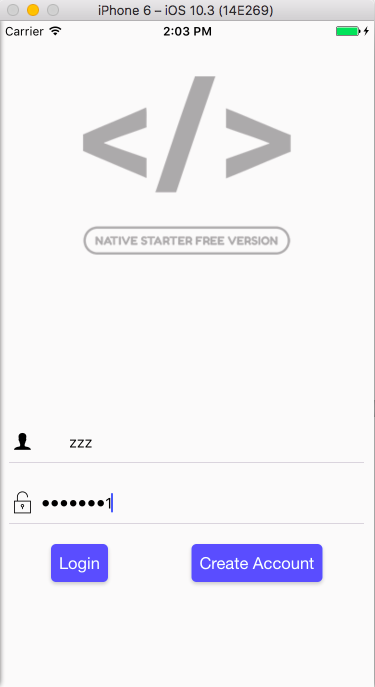
\includegraphics[width=5cm]{./img/mobile.png}
\end{figure}

\begin{figure}[htbp]
\caption{\label{fig:orgedc7f17}
Mobile Functions}
\centering
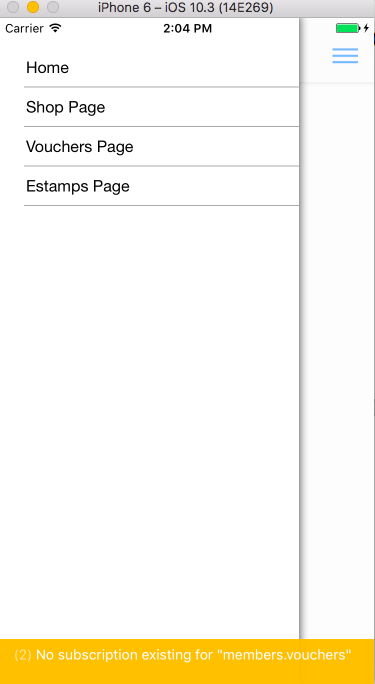
\includegraphics[width=5cm]{./img/mobilefunction.png}
\end{figure}

\subsection{Dashboard}
\label{sec:org48d675d}
\hyperref[fig:orgb704847]{\emph{AdminDashboard}} for the shop holders. They can use this to
add the new customers to their loyalty system and group them to distribute
the \hyperref[fig:org4f8b0d1]{\emph{e-stamps}}, \hyperref[fig:orgbb5aa01]{\emph{e-vouchers}} \hyperref[fig:org90ab7ca]{\emph{create}} and push the \hyperref[fig:orgfa04102]{\emph{promotion notifications}}
\begin{figure}[htbp]
\caption{\label{fig:orgb704847}
Dashboard for the shop holders}
\centering
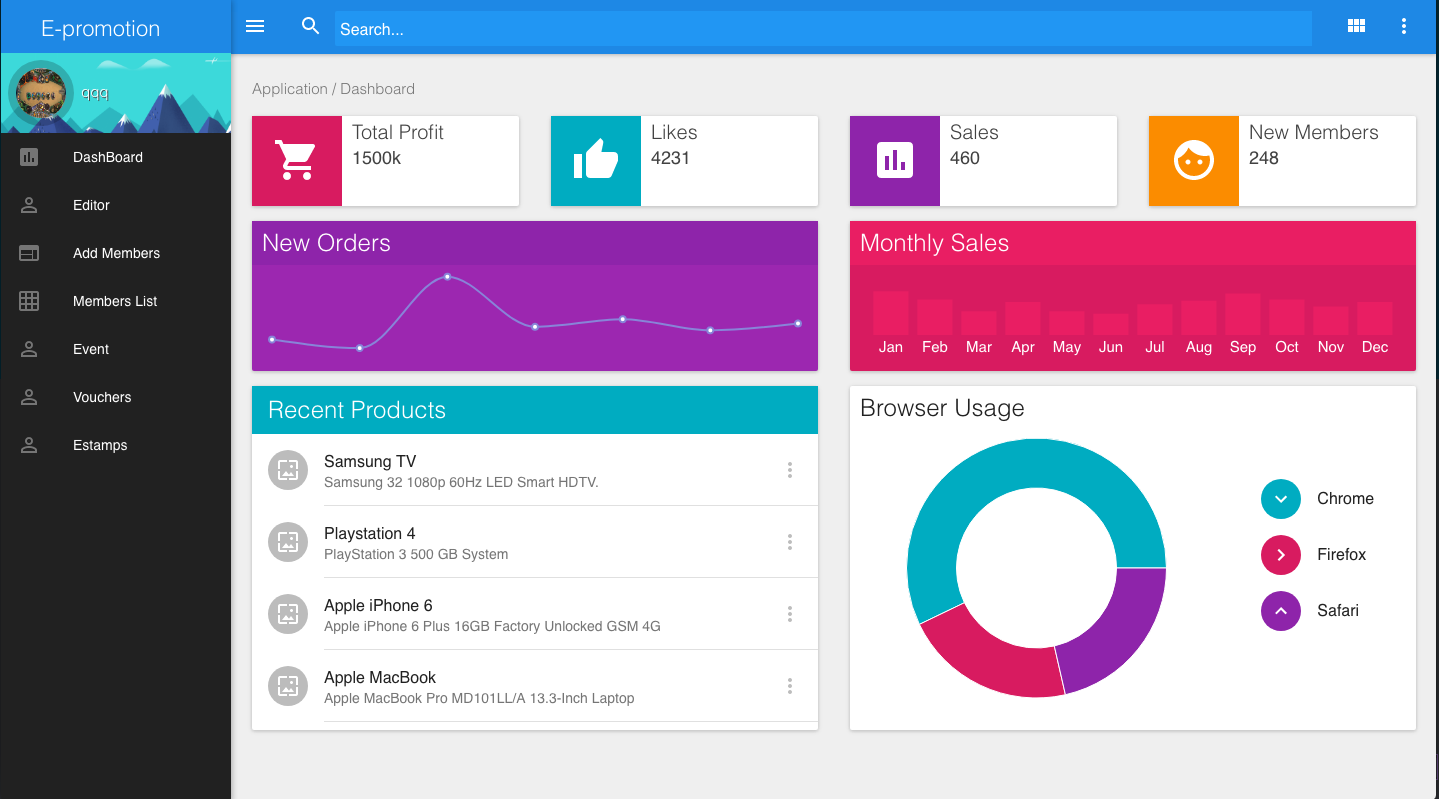
\includegraphics[width=.9\linewidth]{./img/dashboard.png}
\end{figure}

\begin{figure}[htbp]
\caption{\label{fig:org90ab7ca}
Editor to write new notifications}
\centering
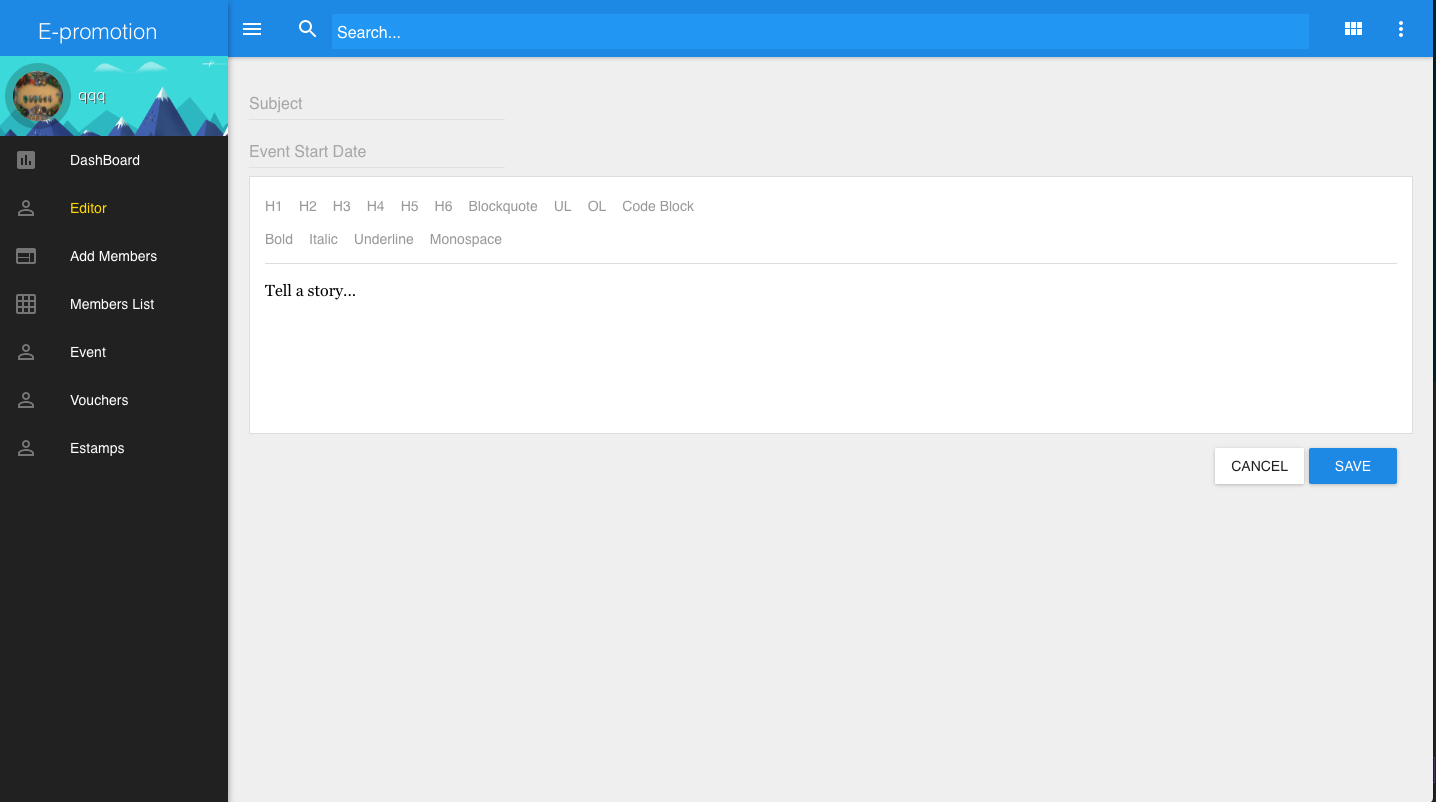
\includegraphics[width=.9\linewidth]{./img/editor.png}
\end{figure}
\begin{figure}[htbp]
\caption{\label{fig:orgbb5aa01}
Form to create new vouchers}
\centering
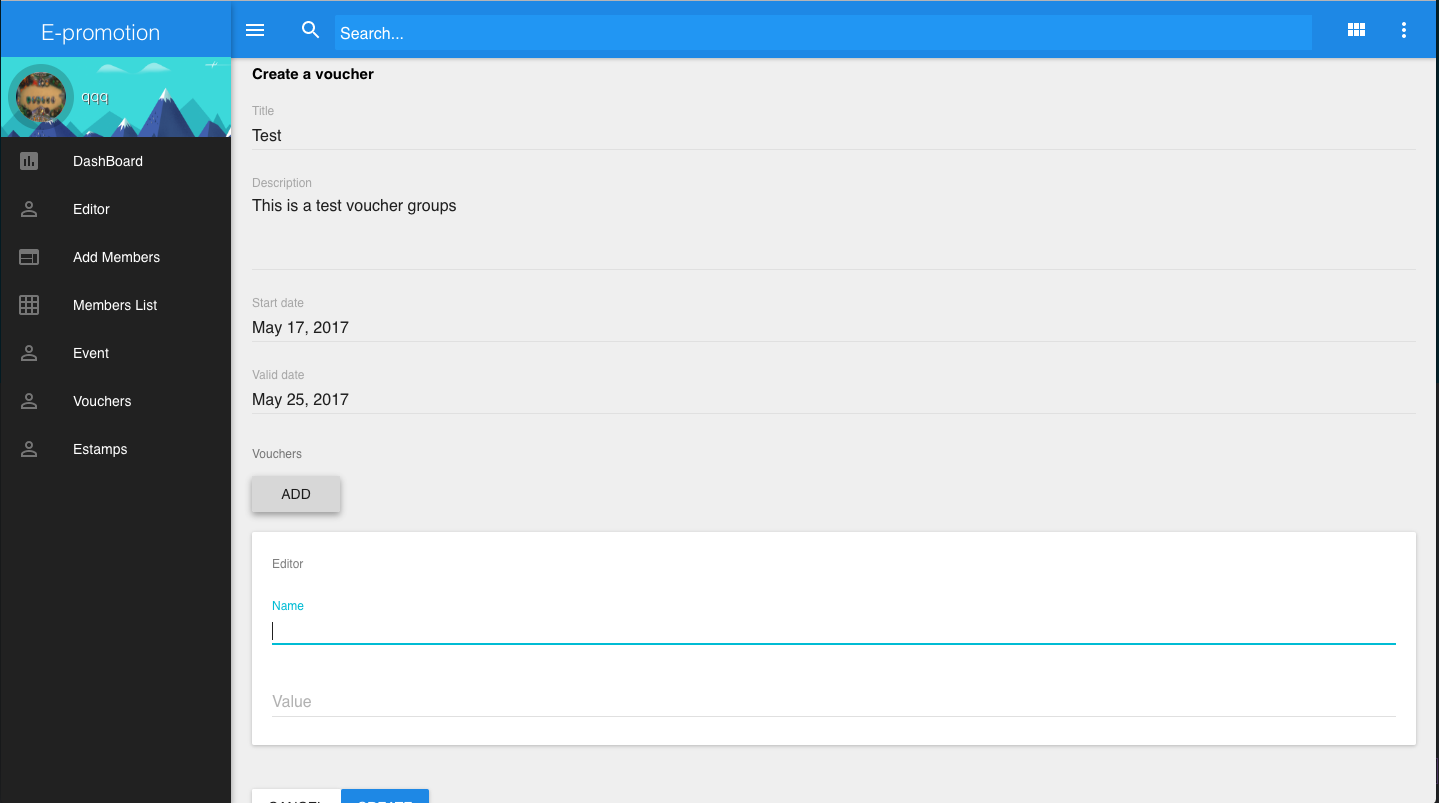
\includegraphics[width=.9\linewidth]{./img/voucher.png}
\end{figure}
\begin{figure}[htbp]
\caption{\label{fig:org4f8b0d1}
Estamps page}
\centering
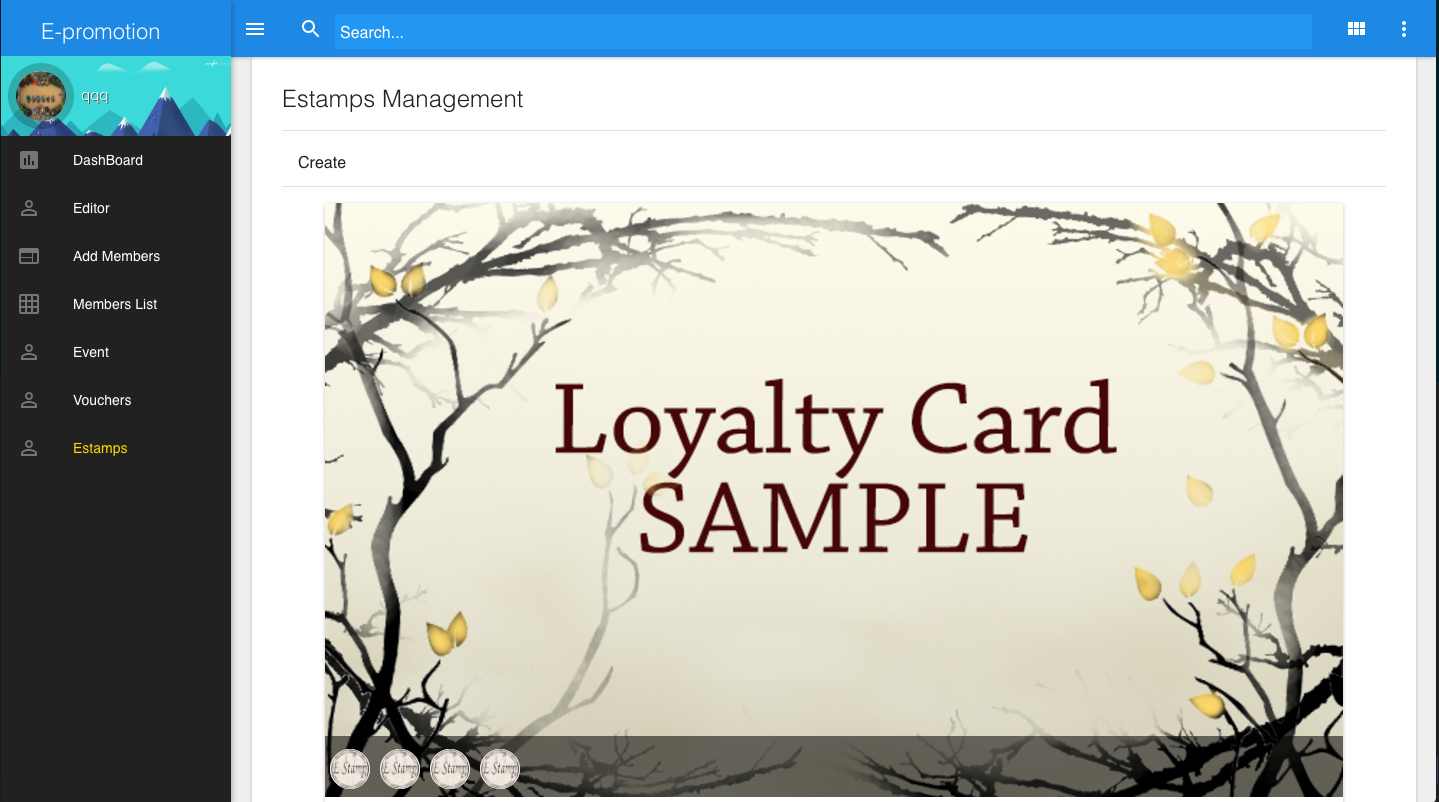
\includegraphics[width=.9\linewidth]{./img/estamp.png}
\end{figure}
\begin{figure}[htbp]
\caption{\label{fig:org07b2067}
Page to add new member}
\centering
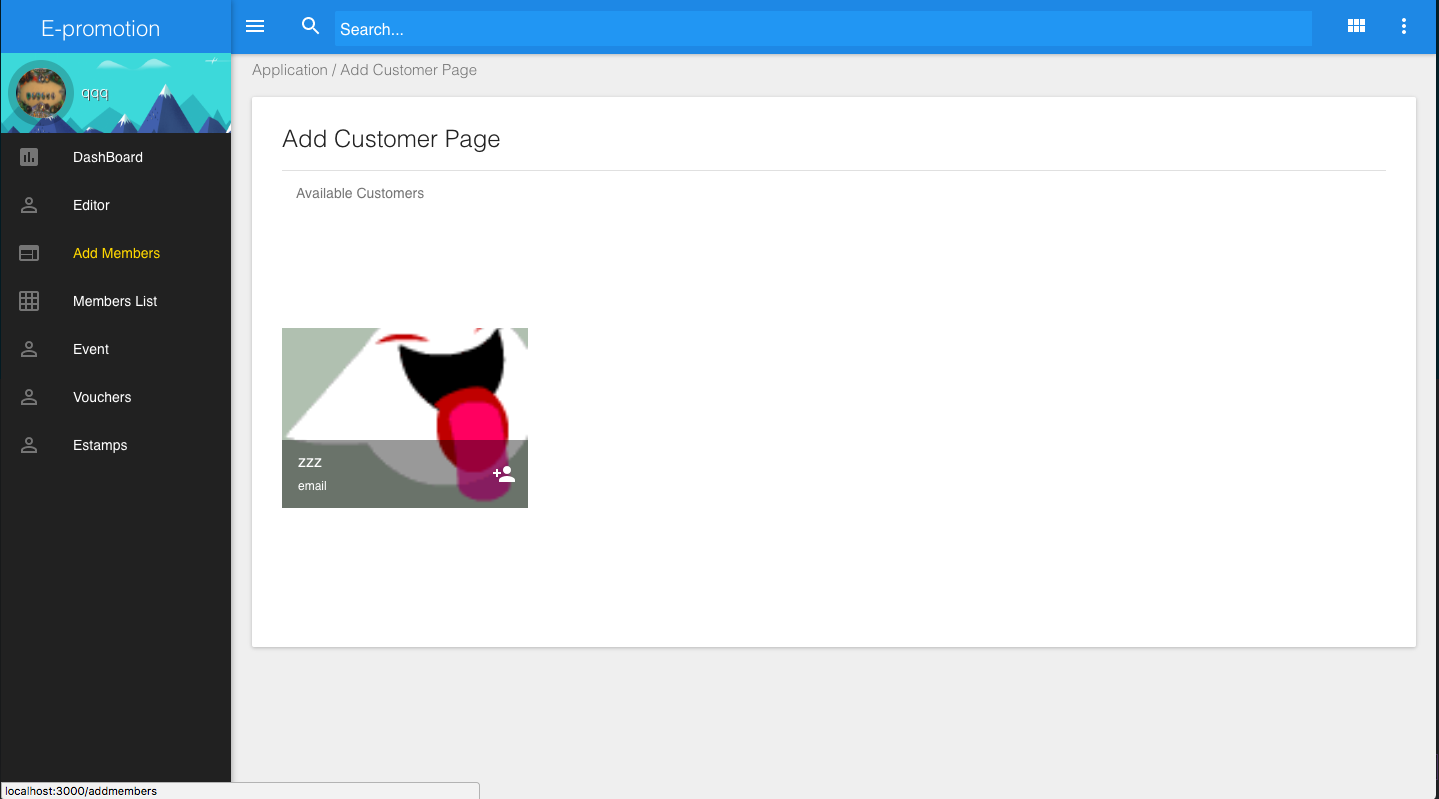
\includegraphics[width=.9\linewidth]{./img/customer.png}
\end{figure}
\begin{figure}[htbp]
\caption{\label{fig:orgfa04102}
Page to distribute vouchers}
\centering
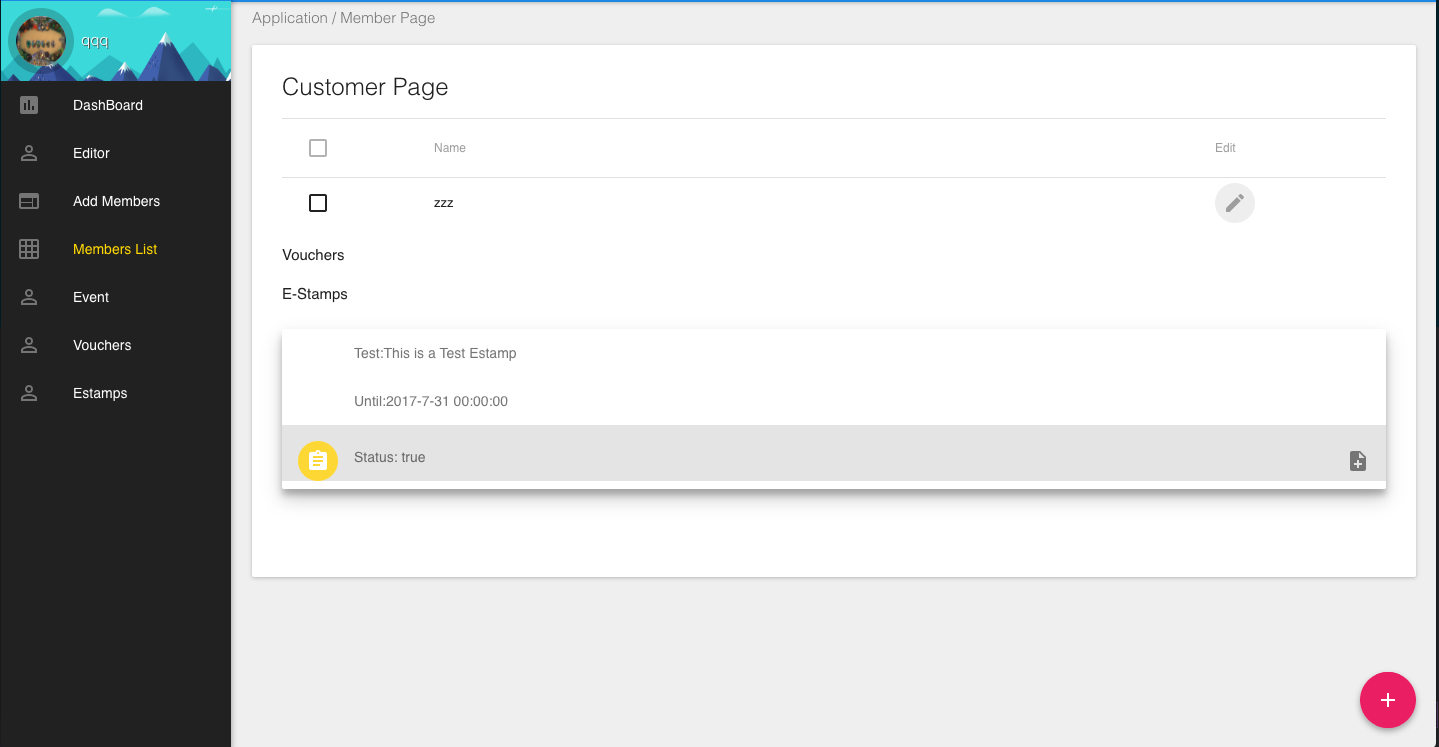
\includegraphics[width=.9\linewidth]{./img/distribute.png}
\end{figure}

\subsection{Review of theory and previous work}
\label{sec:orgbb5dc66}
Below shows all my requirement and the successful implementation during the
internship period.
\subsubsection{System Scope(Functional Requirement)}
\label{sec:org3977c02}

\begin{enumerate}
\item Customer Side
\label{sec:orga5e19e1}

\begin{itemize}
\item $\boxtimes$ \textbf{Basic Feature}
\begin{itemize}
\item $\boxtimes$ User Register System(Third Party Oauth)
\item $\boxtimes$ Browse membership to different shops(Sorting,Ranking)
\item $\boxtimes$ Check the royalty system in shop(Point,E-stamp)
\item $\boxtimes$ Promotion System(Vouchers,Sales notification)
\end{itemize}

\item $\boxtimes$ \textbf{Medium Feature}
\begin{itemize}
\item $\boxtimes$ Redeem gift
\end{itemize}

\item $\square$ \textbf{Advanced Feature}
\begin{itemize}
\item $\square$ E-wallet(Paypel,Wechat-Pay,ALi-Pay)
\item $\square$ E payment deduct voucher value
\end{itemize}
\end{itemize}

\item Merchant Side
\label{sec:orgaa21aa2}

\begin{itemize}
\item $\boxtimes$ \textbf{Basic Feature}
\begin{itemize}
\item $\boxtimes$ Regist Shop
\item $\boxtimes$ Selcet templete from template royalty system
\item $\boxtimes$ Distribute Membership to Customer(IC,Scan QR code)
\item $\boxtimes$ Dashboard to display the info of promotion status
\item $\boxtimes$ Modify shop detail
\end{itemize}

\item $\square$ \textbf{Intemeida Feature}
\begin{itemize}
\item $\boxtimes$ Define Member Teir system Based on points
\item $\square$ Define User Groups
\item $\square$ Api to combine our system to the exitsting Pos Systme
\item $\boxtimes$ Create Voucher
\end{itemize}

\item $\square$ \textbf{Advanced Feature}
\begin{itemize}
\item $\square$ Costumize The vouchers(Animation) and so on.
\item $\square$ Costumize tier metal
\end{itemize}
\end{itemize}
\end{enumerate}


\subsubsection{Execution \& Evolution qualities(Non-functional Requirement)}
\label{sec:org0f08393}

\begin{itemize}
\item $\square$ \textbf{Deploy \& Opertate}
\begin{itemize}
\item $\square$ Docker
\end{itemize}

\item $\square$ Backup

\item $\boxtimes$ Unit Testing

\item $\square$ Pressure Tesing
\end{itemize}

\subsection{Self explore}
\label{sec:orgf98fa74}
I did learn a lot from this internship. Cause it is the first time I am
in charge of a huge project and explore every things the frameworks extra.
So I will talk more on this in different respect.
\subsubsection{Literate writing}
\label{sec:orgc2d442b}
When I start to write documentation, I pay a lot of attention to the iterate
writing. This kind of skills set help me to write documentations, reports,
and academic papers a lots. Because you can write code when you write things
and it gives you a lot of efficiency. I use this skills to write this
reports. The tables of content and the table, figures graphs all
auto-generate. And you can do more. You can find a demo in
\hyperref[fig:org8850b04]{Python Plot}

\begin{verbatim}
import pylab as pl
from numpy import sin, pi, linspace
t = linspace(0, 2*pi, 100)
pl.plot(t, sin(t))
pic = 'img/myfig.png'
pl.savefig(pic)
return 'img/myfig.png'
\end{verbatim}

\url{}
\subsubsection{Category theory}
\label{sec:org8f13b47}
During the last month, I pay a lot time to learn the category mathematics.
Because I find myself lack of this kind of knowledge since I am a electronic
student not computer science. While I decide to be a programmer in the
future. I love programming and I find the category theory help me a lot to
build real world model to a software model.

\texttt{Primitive} : No property
Abstraction
\texttt{Composition}
\begin{figure}[htbp]
\caption{\label{fig:orgce3c6df}
Composition}
\centering
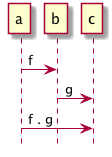
\includegraphics[width=5cm]{img/composition.png}
\end{figure}

\texttt{Identity}
f . id\(_{\text{a}}\)  = f
\begin{figure}[htbp]
\caption{\label{fig:orgab00620}
Identity}
\centering
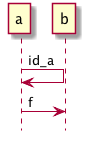
\includegraphics[width=5cm]{img/identity.png}
\end{figure}

\texttt{Associativity}
h . (g . f) = (h . g) . f
\begin{figure}[htbp]
\caption{\label{fig:org778a035}
Associativity}
\centering
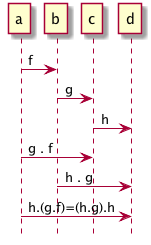
\includegraphics[width=5cm]{img/Associativity.png}
\end{figure}

\texttt{Function} :  A mapping of values to values

\begin{enumerate}
\item Monoid\hfill{}\textsc{NOTE}
\label{sec:org396ecf0}
\textit{[2017-05-09 Tue 18:27]}
mappend maps an element of a monoid set to a function acting on that set

\item Category\hfill{}\textsc{NOTE}
\label{sec:orgae611ff}
\textit{[2017-05-09 Tue 23:17]}
\texttt{Kleisli category}  a category based on a monad.
\item Initial Object\hfill{}\textsc{NOTE}
\label{sec:org0502608}
\textit{[2017-05-09 Tue 23:36]}
The initial object is the object that has one and only one morphism going to any object in the category.

\newpage
\end{enumerate}
\section{Chapter Three}
\label{sec:org3c21cce}
\subsection{Summary and Conclusion}
\label{sec:org2bd2122}
I explore a lot good stuff during the internship, and make lots of life change
movement. Below show all my tools chains and they working together fantastic.
\begin{table}[htbp]
\caption{\label{tab:orgcbf30eb}
My life Change tools}
\centering
\begin{tabular}{ll}
Usage & Application\\
\hline
Email & imap:mbsync smtp:msmtp\\
Crypt & gnu2\\
Editor & Emacs, neovim\\
Ide & Intellij\\
Shell & Zsh\\
Shell manager & Oh-my-zsh\\
Searcher & fasd, ag\\
Termial & Iterm2\\
Chat & QQ, Wechat, Erc\\
Presentation & Reveal.js\\
GTD & Org Agenda\\
Notes & Onenote -> Org Mode\\
Graph Draw & Plantuml, Ditaa, Gnuplot\\
Documentation View & Dash\\
Book Writing & Gitbook\\
Finance & Ledger\\
Auto Deploy & Pm2, Docker\\
Academic Writing & Pandadoc, Org mode\\
Desktop & Xmonad\\
\end{tabular}
\end{table}

I did love and enjoy the key-bindings of vim, from the day I switch from the emacs, but I switch back shortly because of the 2 main reasons.
\begin{enumerate}
\item Emacs plugins works on my windows but the my vim got some problem and I have to dirty my configuration files so much to fixed.
\item I need to use playframework for development and the emacs support ensime very well.
\end{enumerate}

I move from emacs to vim then to neovim and now I am using the spacemacs, I think the configuration for everyone will become the same after long period of learning and copying from others, so it is good to give the community driven software a try.

Besides that, I also earn lots of the develop experience in the web area. And I
have the confidence to do well in the final year project.

\newpage
\section{References}
\label{sec:orgc5423b9}
\subsection{My Book List}
\label{sec:org18f4aa9}
\begin{enumerate}
\item {\bfseries\sffamily DONE} \href{http://learnyouahaskell.com/chapters}{Learn Your Haskell A Great Good }
\label{sec:org0f15ba0}

\item {\bfseries\sffamily HOLD} Introduction to algorithms\hfill{}\textsc{HOLD}
\label{sec:org1ab4282}
\begin{itemize}
\item State "HOLD"       from "TODO"       \textit{[2017-05-04 Thu 13:12] } \\
Stop at black and red tree
\end{itemize}
\item {\bfseries\sffamily WAITING} Computer System (A Programmer Perspective)\hfill{}\textsc{WAITING}
\label{sec:org4606690}
\begin{itemize}
\item State "WAITING"    from "TODO"       \textit{[2017-05-04 Thu 10:33] } \\
Boring
\end{itemize}
\newpage
\end{enumerate}
\section{Appendix A}
\label{sec:org91b4523}
\subsection{Gantt Table}
\label{sec:orge216bd9}
\begin{verbatim}
Project starts the 9th of Jan 2017
[Research and Learn] lasts 31 days and is colored in Lavender/LightBlue
[Prototype Design] lasts 31 days and is colored in Coral/Green
[Prototype Design] starts 14 days after [Research and Learn]'s end
[Test prototype] lasts 31 days and is colored in Red
[Test prototype] starts 2 days before [Prototype Design]'s end
[Write tests] lasts 5 days and ends at [Prototype Design]'s end
[Document] lasts 31 days and ends at [Write tests]'s start
[Init and write tests report] is colored in Coral/Green
[Init and write tests report] starts 31 day after [Test prototype]'s start
[Self explore] lasts 25 days and is colored in Black
[Self explore] starts 4 days before [Init and write tests report]'s end
\end{verbatim}

\begin{figure}[htbp]
\caption{\label{fig:orgf349192}
Gantt Table}
\centering
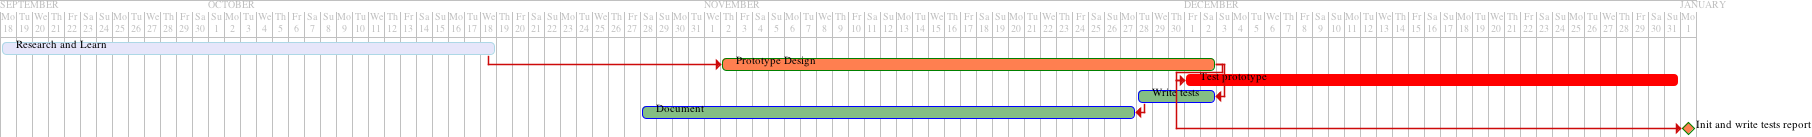
\includegraphics[width=.9\linewidth]{img/gantt.png}
\end{figure}
\end{document}